\section{Tecnologías}

\subsection{Mongo}

MongoDB es una base de datos NoSQL (no solo SQL) orientada a documentos. Almacena
datos en una representación binaria llamada BSON (Binary JSON), la cual extiende
las capacidades de un objeto JSON (JavaScript Object Notation) para representar
tipos de datos como enteros, punto flotante, fechas, datos binarios, arreglos y sub-documentos o
documentos embebidos. Cada documento pertenece a un grupo llamado colección, los cuales son el
equivalente a las tablas de una base de datos relacional.

MongoDB posee un conjunto de  características que permiten la escalabilidad de una aplicación, entre ellas,
provee la habilidad e implementar la distribución geográfica de datos (sharding). Esto permite a la
base de datos ser escalada de forma horizontal con el uso de un conjunto de componentes de hardware o mediante
de la nube (cloud).

Adicionalmente, MongoDB esta diseñado para ser ejecutado en un sistema de múltiples nodos, por lo tanto,
en la presencia de un escalamiento horizontal, incluye la capacidad para la replicación
y sincronización de datos entre todos los componentes del sistema. De esta manera se garantiza la posibilidad
de implementar un servicio con alta disponibilidad \cite{10}.

\subsubsection{Replicación}

La replicación permite la redundancia de datos y el aumento de disponibilidad de los mismos en aplicaciones distribuidas.
Hace uso de múltiples servidores conectados entre sí y genera una replica de los datos en cada uno de ellos, de
esta manera se obtiene cierto nivel de tolerancia a fallos en caso de que un servidor de base de datos falle. 
También es posible mantener copias adicionales para propósitos específicos como recuperación en casos de desastre,
reportes o respaldos \cite{11}.

En MongoDB se hace uso de grupos de replica (replica sets) para almacenar las copias de datos en múltiples
servidores de base de datos. Un grupo de replica previene los tiempos de inactividad de la base de datos
en caso de errores y ayuda a escalar las operaciones de lectura. La recuperación de un miembro del grupo de
replica se realiza de forma automática. En un grupo de replica cualquier miembro puede actuar como nodo principal 
y el resto como secundario, por lo tanto, en caso de fallas de red o de hardware, un miembro del grupo
puede tomar el puesto de nodo primario después de haber sido elegido siguiendo un conjunto de reglas predefinidas.

Un grupo de replicas esta conformado por un nodo principal que realizara todas las operaciones de escritura, múltiples nodos 
secundarios y un nodo arbitro opcional, tal cual como lo muestra la siguiente figura:

\begin{figure}[H]
	\centering
		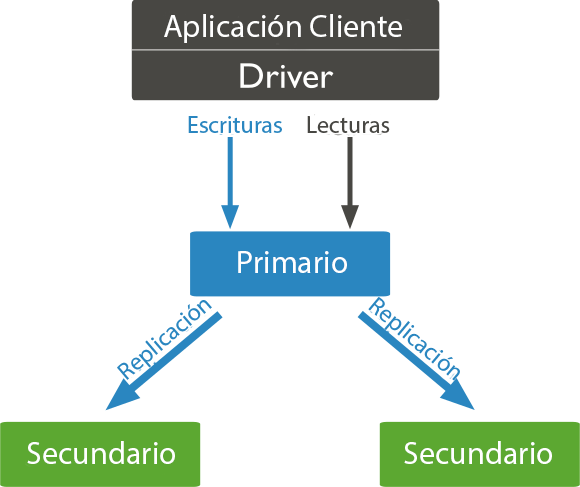
\includegraphics[width=.6\textwidth]{figures/replicas}
	\caption{Componentes de un grupo de replicas en MongoDB y su interacción con una aplicación cliente.}
	\label{fig:replicas}
\end{figure}

Para poder crear estos grupos es necesario tener un mínimo de tres nodos y escalar en números impares. Esto se 
debe a que cuando los componentes del grupo realicen la votación para elegir el nodo principal, se elimina la posibilidad de un
empate y el ganador es elegido de inmediato. 

En la siguiente figura se puede observar como los nodos del grupo se envían mensajes de diagnostico (heartbeats) para determinar
si sus vecinos son accesibles o no. En caso de que uno de estos heartbeat no obtenga una respuesta en 10 segundos, se marca dicho
destinarlo como inaccesibles.

\begin{figure}[H]
	\centering
		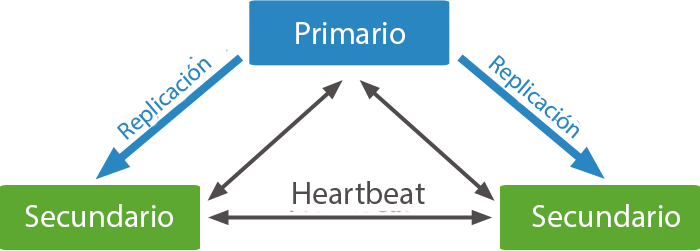
\includegraphics[width=.6\textwidth]{figures/heartbeat}
	\caption{Hearbeats en un grupo de replicación de MongoDB.}
	\label{fig:heartbeat}
\end{figure}


Los nodos secundarios se encargan de leer los datos presentes en el nodo primario y crear sus propia replica o copia del mismo.
Si, por alguna razón, el nodo primario deja de estar disponible, un nodo secundario elegible ejecutará una votación para 
elegir el siguiente nodo primario, tal como lo muestra la figura \ref{fig:failover}.
El primer nodo secundario en llevar a cabo la elección y recibir la mayoría de los botos se convierte en el nuevo nodo primario.


\begin{figure}[H]
	\centering
		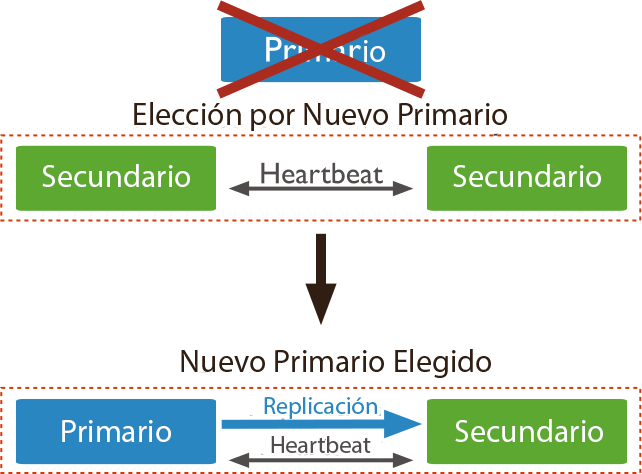
\includegraphics[width=.6\textwidth]{figures/failover}
	\caption{Proceso de elección de nuevo nodo primario.}
	\label{fig:failover}
\end{figure}


\subsubsection{Particiones}

El proceso de partición (sharding) es un método de escalamiento horizontal que distribuye datos entre múltiples maquinas.
Cada conjunto de datos alojado en una maquina es llamado partición (shards), y su acceso es completamente transparente
para las aplicaciones. Este método permite atacar las limitaciones de hardware provenientes del uso de un solo servidor, tales como
los cuellos de botella o capacidad de almacenamiento \cite{13}.

En MongoDB, un grupo de partición (sharded cluster) consiste de tres componentes:

\begin{itemize}
\item Partición: Cada partición contiene un subconjunto de los datos y pueden ser implementados como un grupo de replica.

\item mongos: mongos es un servicio que actuá como interfaz entre las aplicaciones cliente y el grupo de partición, también es llamado
query router.

\item Servidores de Configuración: Los servidores de configuración almacenan meta datos y los atributos de configuración del cluster, y
al igual que las particiones, también pueden ser implementados como un grupo de replica.
\end{itemize}

En la siguiente figura se puede apreciar los componentes del cluster de particiones y la interacción entre los mismos:

\begin{figure}[H]
	\centering
		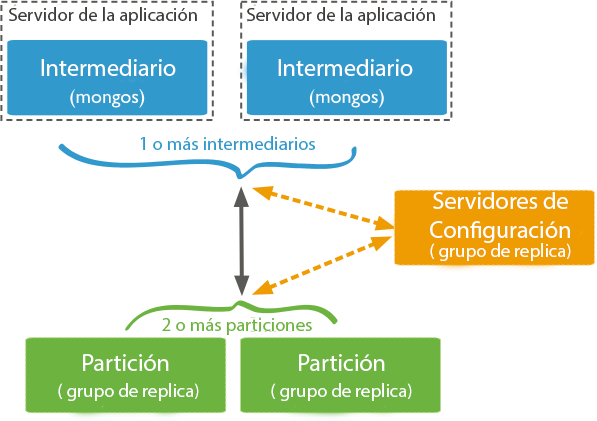
\includegraphics[width=.7\textwidth]{figures/sharding}
	\caption{Componentes de un cluster de particiones.}
	\label{fig:sharding}
\end{figure}

Para distribuir los documentos de un colección es necesario el uso de una llave de partición (shard key). Un shard key es uno o 
múltiples campos inmutables que comparten todos los documentos de una colección. Una colección particionada solo puede tener un shard key
y la misma no puede ser cambiada después de haberse ejecutado el proceso de sharding.

MongoDB genera particiones de datos a nivel de colección, distribuyendo los documentos de una colección entre los miembros
del cluster de particiones. Una base de datos puede tener una combinación de colecciones particionadas y no particionadas.
Las colecciones particionadas son distribuidas entre cada partición del cluster, mientras que las colecciones no particionadas son
almacenadas en una partición especial llamada primaria.

El acceso a una base de datos particionada en MongoDB es completamente transparente para cualquier aplicación de cliente, tan
solo es necesario saber la dirección IP o nombre del equipo (hostname) y el puerto en el cual se ejecutará el query router.
La siguiente figura detalla la interacción entre una aplicación de cliente con una base de datos MongoDB con particiones:

\begin{figure}[H]
	\centering
		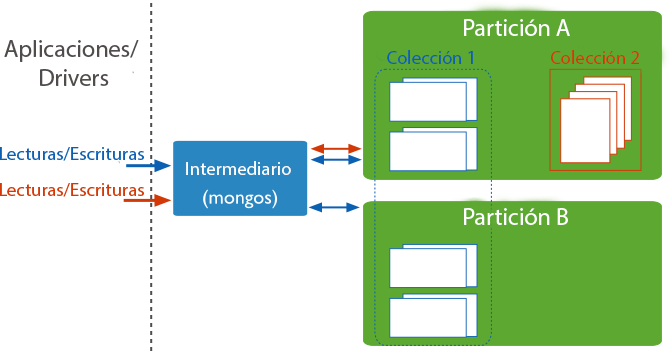
\includegraphics[width=.7\textwidth]{figures/sharding_apps}
	\caption{Interacción entre una aplicación cliente y una base de datos MongoDB particionada.}
	\label{fig:sharding_apps}
\end{figure}

MongoDB ofrece múltiples estrategias o políticas de particionamiento que permiten a un administrador de base de datos
o desarrollador distribuir los datos entre los miembros del cluster.

\begin{itemize}

\item Range Sharding. Los documentos son divididos en rangos contiguos determinados por el valor del shard key. Se toma el valor 
mínimo y máximo de todos las particiones y se generan N grupos, ordenados de menor a mayor por el shard key y separados por rangos,
tal cual se puede observar en la siguiente figura:

\begin{figure}[H]
	\centering
		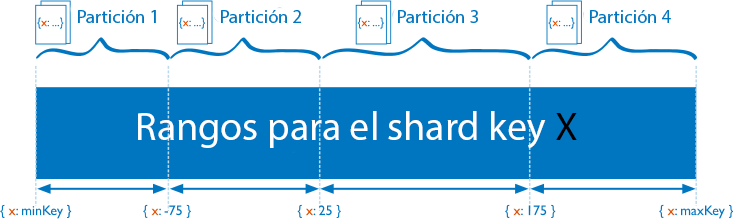
\includegraphics[width=.7\textwidth]{figures/ranged_sharding}
	\caption{Range Sharding de datos en MongoDB.}
	\label{fig:ranged_sharding}
\end{figure}

\item Hash Sharding. Los documentos son distribuidos acorde al valor del hash MD5 del shard key. Una vez calculado el valor del hash, se
dividen los datos en subgrupos separados en rangos. Este método garantiza la distribución uniforme de los documentos entre las particiones.
MongoDB es quien calcula el valor del hash, por lo que las aplicaciones que interactúen con la base de datos no necesitan llevar a cabo este paso. Un ejemplo de esto se puede apreciar en la siguiente figura:

\begin{figure}[H]
	\centering
		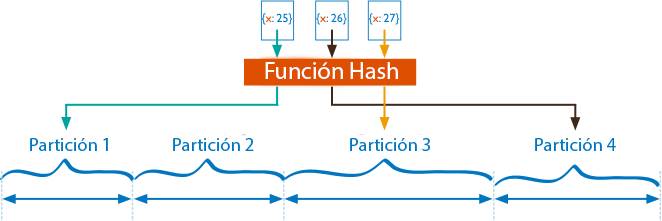
\includegraphics[width=.7\textwidth]{figures/hashed_sharding}
	\caption{Hashed Sharding de datos en MongoDB.}
	\label{fig:hashed_sharding}
\end{figure}

\item Zone Sharding. Provee las herramientas para la definición de las reglas que definen el lugar en que serán almacenados los datos
en el cluster. Se crean zonas de datos particionados basados en el shard key, y es posible asociar cada zona con uno o más particiones
del cluster. Zone Sharding permite establecer políticas en donde se puede almacenar y localizar datos por región geográfica, por
servicios específicos de una aplicación, e incluso por la configuración de hardware en caso de tener una arquitectura de almacenamiento
por capas.

\begin{figure}[H]
	\centering
		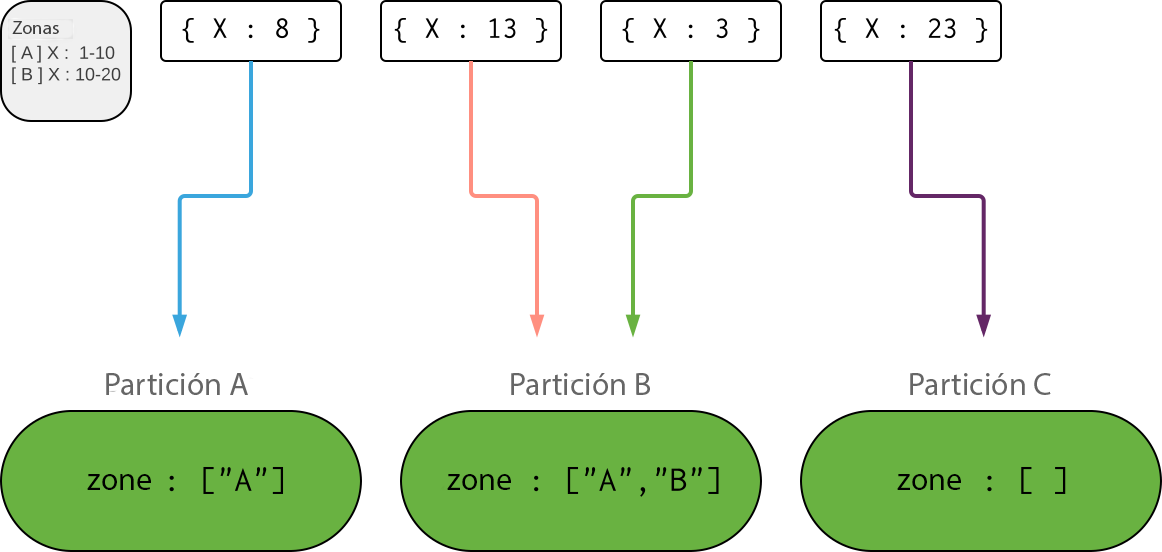
\includegraphics[width=.9\textwidth]{figures/zone_sharding}
	\caption{Zone Sharding de datos en MongoDB.}
	\label{fig:zone_sharding}
\end{figure}

\end{itemize}


\subsection{Celery}

\subsection{RabbitMQ}

\subsection{Flask}

% Is this subsection necessary?
\subsection{Wikipedia API}

